\section{Results}
\subsection{Effects of Learning Rate}
The first simulations were run with learning rate values of $0.8$, $0.5$, $0.2$ and $0.0$, corresponding to the inexperienced, mixed-experienced, experienced and non-learning cops. Following, the simulation with a decreasing learning rate, starting at $0.8$ was run. The mean performance and standard deviation (SD) can be found in \autoref{tab:ResultsCur}. 

\begin{table}[!ht]
\begin{center}
\begin{tabular}{l r  r}
$\lambda$ &  \# epochs (SD) & success (SD)\\
\hline
0.0 & 17.79 (1.623) & 0.25 (0.036) \\
0.2 & 17.66 (2.194) & 0.25 (0.036) \\
0.5 & 18.12 (2.502) & 0.25 (0.036) \\
0.8 & 18.45 (2.288) & 0.25 (0.036) \\
<0.8 & 17.53 (1.825) & 0.25 (0.036) \\
\hline
\end{tabular}
\caption{The amount of epochs necessary to finish and the success of the simulation for the cop-teams with different levels of experience. }
\label{tab:ResultsCur}
\end{center}
\end{table}
A Repeated Measure Analysis of Variance (RM-ANOVA) showed that there was a main effect on learning rate for the amount of epochs (F(4,4995) = 31.204, p < 0.001), but not for the success value (F(4,4995) = 2.306, p = 0.054). Post-hoc pairwise comparison, using Bonferroni correction, showed that the 0.0, 0.2 and <0.8 simulations were significantly faster compared to the 0.5 and 0.8 simulation. This suggests that a(n ultimately) lower learning rate and, therefore, more stable performance, ensure better performance. Note, however, that the difference is at most 1 epoch, meaning that the effect is not very large. 

In \autoref{tab:ResultsBias} the mean amount of epochs and the mean success of the five conditions are shown for both the incapacitate- and save-biased cops. The first value that deserves some explanation is the speed of the incapacitate-biased cops that do not learn ($\lambda = 0.0$). In this situation there is 90\% possibility that the cops will incapacitate a hostile in every step. Even when there are no more hostiles left, the cops will keep trying to incapacitate a hostile most of the time. Saving civilians will only occur once every ten times and will, therefore, take a very long time. In the statistical analysis, this scenario was excluded. 

\begin{table}
\begin{center}
\begin{tabular}{l r  r | l r  r}
$\lambda$ &  \# epochs (SD) & success (SD) & $\lambda$ &  \# epochs (SD) & success (SD)\\
\hline
0.0 & 350.58 (49.631) & 0.30 (0.050) & 0.0 & 9.32 (0.864) & 0.15 (0.032)\\
0.2 & 19.89 (2.690) & 0.39 (0.026) & 0.2 & 13.41 (1.893) & 0.17 (0.039)\\
0.5 & 20.64 (2.354) & 0.37 (0.027) & 0.5 & 14.57 (1.936) & 0.17 (0.039)\\
0.8 & 20.64 (2.344) & 0.35 (0.029) & 0.8 & 14.90 (1.937) & 0.17 (0.039)\\
<0.8 & 20.28 (2.145) & 0.37 (0.027) & <0.8 & 11.55 (1.214) & 0.16 (0.035)\\
\hline
\end{tabular}
\caption{The amount of epochs necessary to finish and the success of the simulation for the cop-teams with different levels of experience. The cops have a bias for incapacitating (left) and saving (right).}
\label{tab:ResultsBias}
\end{center}
\end{table}
For the incapacitate-biased cops a significant main effect was found on speed (F(3,3996) = 22.365; p < 0.001) and success (F(3,3996) = 21.587; p < 0.001). Post-hoc analysis with Bonferroni correction showed that the 0.2 learning rate condition scored significantly better than the <0.8 condition on both performance measures. The <0.8 condition, in turn, scored significantly better than the 0.5 and 0.8 conditions, again suggesting that in the end an ultimately lower learning rate ensures a higher and more stable performance. 

For the save-biased cops a main effect was found on speed (F(4,4995) = 2025.756; p < 0.001), but not on success (F(4,4995) = 0.960; p = 0.428). Post-hoc analyses showed that the the learning rate conditions have the following ordering in speed: 0.0, <0.8, 0.2, 0.5, 0.8, with only significant (p<0.001) differences. Again, less variable behavior is associated with higher speed. 

These differences that were found can be considered negligible. Therefore, it was interesting to see whether learning affected success and speed at all. Not over all the 1000 simulations, nor over the first 100 (separate for each bias), did speed and success significantly change (p > 0.05), except for the success during saving over 100 simulations (F(98,396) = 1.392; p = 0.015) and the success of incapacitating over 1000 simulations (F(999,4000) = 1.101; p = 0.024). Because of the small effects and the inconsistency (the lack of significance over a longer and shorter time period) these results can be considered negligible. This suggests that learning any behavior in this particular multi-agent system, which occurs over time and over simulations, does not or hardly affect large group performance. 

\subsection{Effects of Bias}
The results in \autoref{tab:ResultsCur} and \autoref{tab:ResultsBias} showed another interesting pattern. It appeared that there was an inverse relation between speed and success given the two actions. Whereas the no-bias simulation shows intermediate results ($m_{epochs} = 17.91$; $SD_{epochs} = 2.136$; $m_{success} = 0.23$; $SD_{success} = 0.075$), the incapacitate-bias simulation shows a low speed ($m_{epochs} = 20.36$; $SD_{epochs} = 2.41$) and high success ($m_{success} = 0.33$; $SD = 0.111$), as opposed to the save bias ($m_{epochs} = 12.75$; $SD_{epochs} = 2.641$; $m_{success} = 0.18$; $SD_{succes} = 0.143$). An RM-ANOVA showed that these differences were significant (p < 0.001). Note that for the incapacitate-bias, the no-learning cops were again excluded. These results suggest that a bias for an action has a large effect on the success of mitigating civil violence.

\begin{figure}[H]

\centering
\begin{subfigure}[b]{0.62\textwidth}
        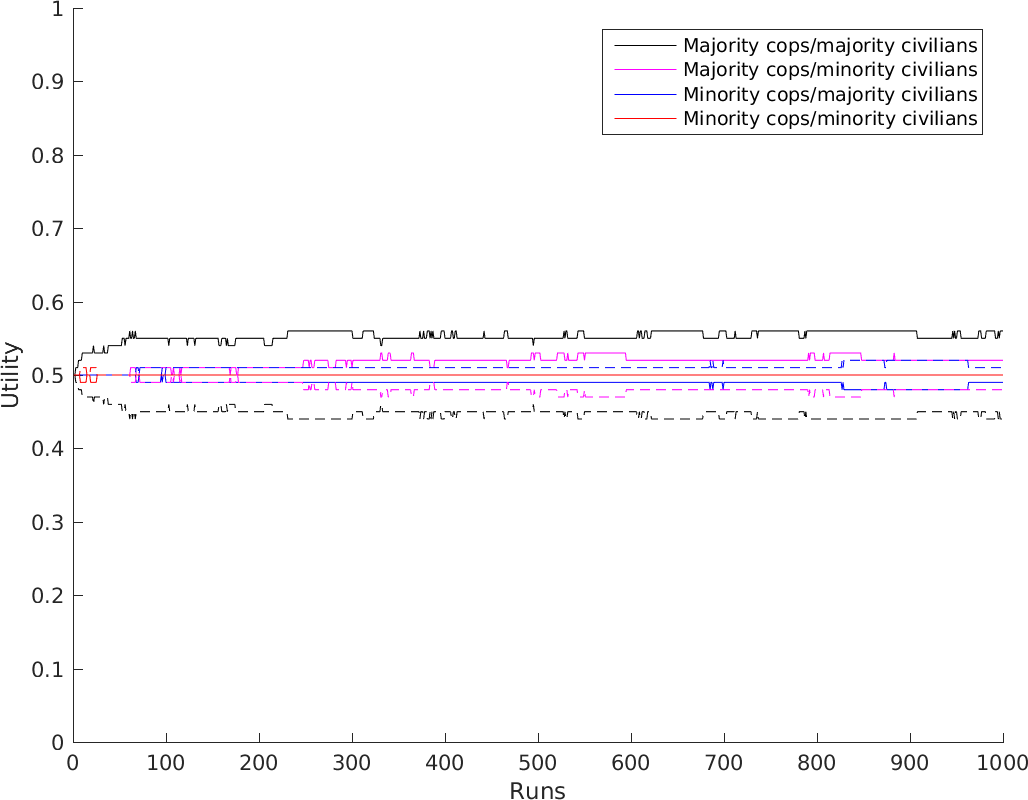
\includegraphics[width=\textwidth]{./pictures/Utility05NoBias.png}
        \caption{Utility for no-biased cops}
        \label{fig:utNoBias}
    \end{subfigure}
    \begin{subfigure}[b]{0.62\textwidth}
        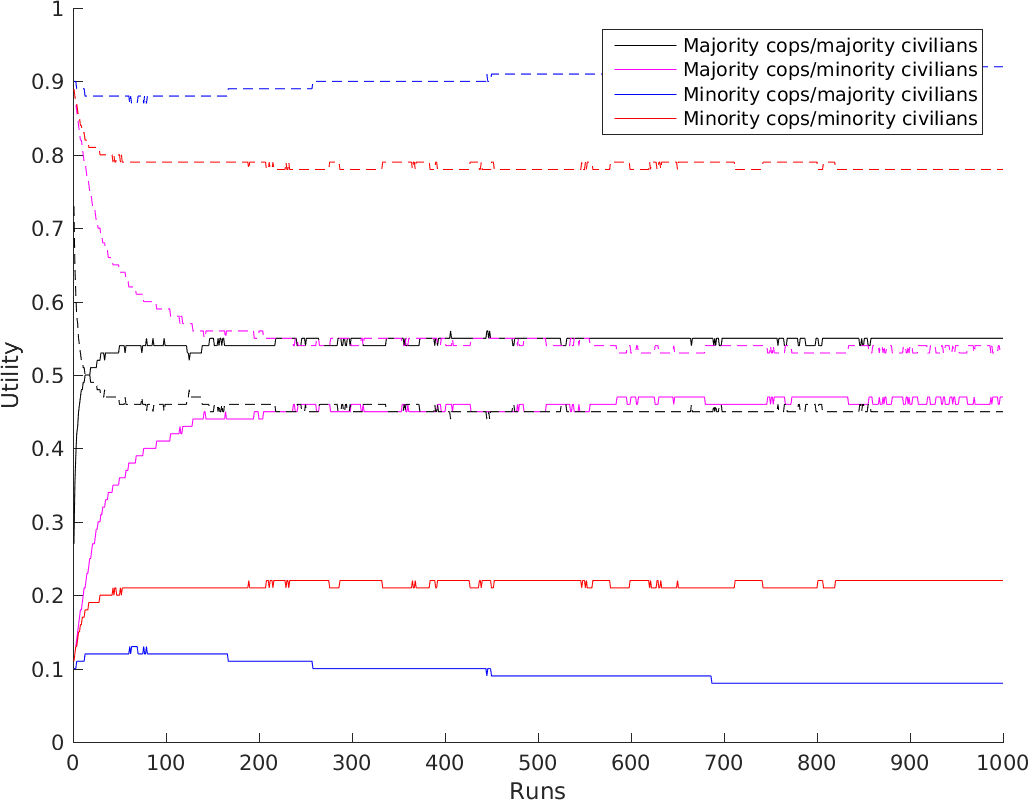
\includegraphics[width=\textwidth]{./pictures/Utility05Shoot}
        \caption{Utility for shoot-biased cops}
        \label{fig:utShoot}
    \end{subfigure}
    \begin{subfigure}[b]{0.62\textwidth}
        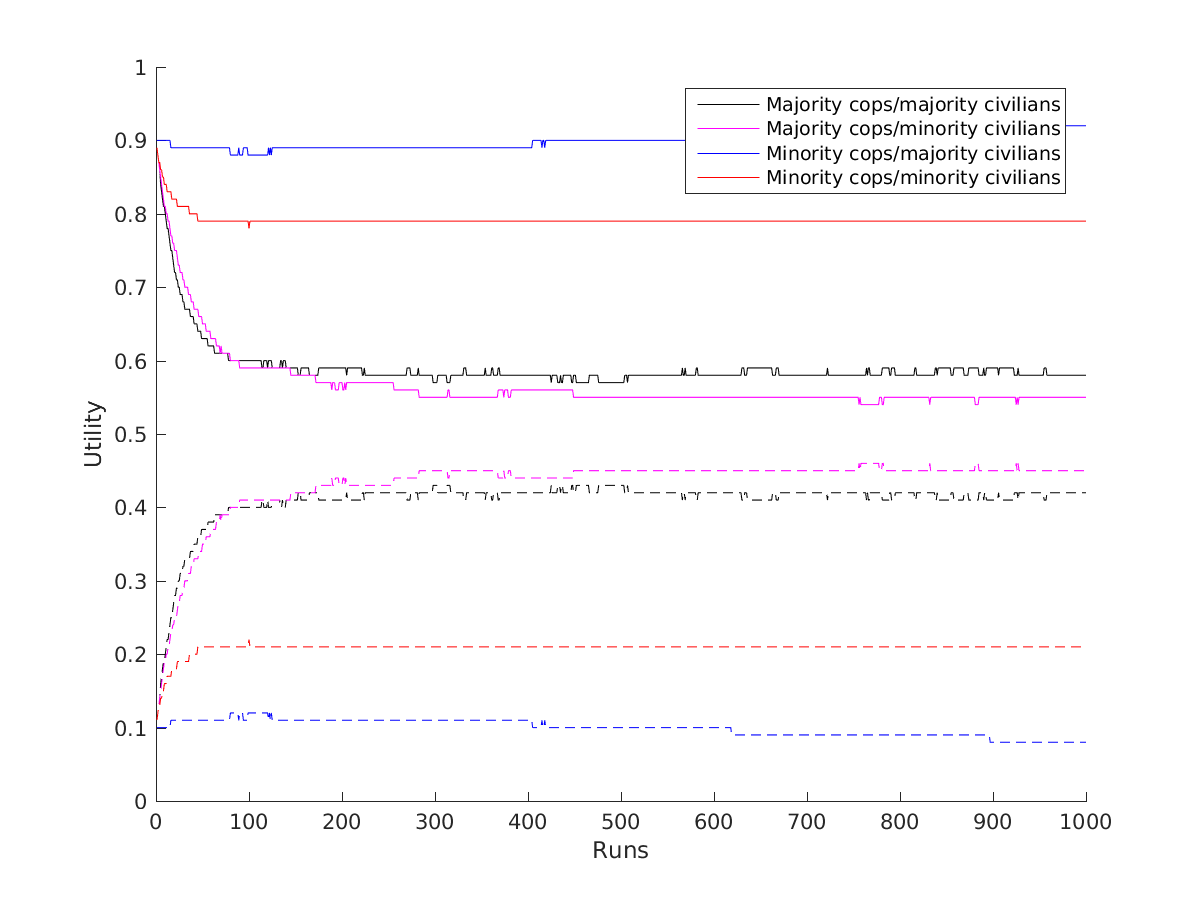
\includegraphics[width=\textwidth]{./pictures/Utility05BiasSave}
        \caption{Utility for save-biased cops }
        \label{fig:utSave}
    \end{subfigure}
\caption{Convergence of utilities for all bias simulations, $\lambda = 0.5$. Dashed lines represent shooting, and solid lines saving. }
\label{fig:utilities}
\end{figure}
In \autoref{fig:utilities}, we show how the biases evolve over time with a medium learning rate ($\lambda = 0.5$). In this figure, the global mean utility for the different actions in the different situations is depicted for all three bias conditions. As is true for all other learning-cop groups, the utilities will converge towards a value of 0.5, though some bias will still exist. Individual agents do show preferences in particular situations, but averaged over all cops, a mixed strategy of saving and shooting appears to be the preferred approach. When the cops are outnumbered by hostiles (the red and blue lines), it does show little changes regardless of the bias. This may indicate that little is learned because the hostiles take out the cops rather quickly. 


